
\section{Vergleich der klassischen mit der bayesischen Methode}
\label{MUFklassischvsbayes}

Als nächstes wollen wir zeigen, dass für die \glqq gutmütigen\grqq ~Fälle, für die das
Gesetz der Mess\-un\-sicher\-heits\-fort\-pflanz\-ung anwendbar ist, die Berechnung des vollständigen
Ergebnisses unter Verwendung der Methode der bayesischen Statistik, deren Konzept wir in
Abschnitt \ref{bayeskonzept} vorgestellt haben, im wesentlichen dasselbe
Resultat liefert wie unter Verwendung des Fort\-pflanz\-ungs\-gesetzes.

Wir betrachten ein Beispiel, bei dem irgendeine physikalische Größe zu messen ist.
Dabei werde ein Gerät bzw.\ Sensor verwendet, dessen Funktionsprinzip auf einem
physikalischen Effekt beruht und dadurch die Größe so erfasst,
dass als direkte Messgröße eine Spannung in Volt angezeigt wird. Dies kann beispielsweise
die Messung einer Temperatur sein, in der das Phänomen, dass sich ein elektrischer
Widerstand proportional zur Tempertur verändert und die Widerstandsänderung über die
Änderung der elektrischen Spannung, die über dem Widerstand abfällt, bestimmt wird.
Dies kann beispielsweise eine Stufenhöhe sein, die mit Hilfe eines induktiven Wegaufnehmers
gemessen wird, der auf dem Phänomen beruht, dass sich die Induktivität einer Spule in Abhängigkeit
von der  Position ihres Ferritkerns verändert. Es sind viele Beispiele denkbar. Sensoren
sind oft so konzipiert, dass sie ein physikalisches Phänomen nutzen und zur elektronischen
Erfassung der zu messenden Größe als direkte Größe ein Messsignal in Form einer elektrischen
Spannung liefern.

Wir wollen im folgenden ganz allgemein die indirekte Messgröße mit $Y$
bezeichnen und uns auf keine physikalische Einheit festlegen, sondern diese allgemein nur
\glqq Einheit\grqq ~nennen. Das Modell, das wir betrachten, ist wie folgt: Das rohe Messsignal,
das als Spannung $U$ bzw.\ direkte Größe $X_\mathrm{M}$ vorliegt, ist über
einen Kalibrierfaktor $K$ bzw.\ eine direkte Größe $X_\mathrm{K}$
in die physikalische Einheit der indirekten physikalischen Größe $Y$ umzurechnen.
Der Index M steht hier für Messung und der Index K für Kalibrierfaktor.

Die indirekte Größe $Y$ habe irgendeine physikalische Einheit $\mathrm{E}$
\begin{equation}
Y \; = \; f(X_\mathrm{K}, X_\mathrm{M})  \; = \; X_\mathrm{K} \, X_\mathrm{M}
\end{equation}
und die beiden direkten Größen $X_\mathrm{M}$ und $X_\mathrm{K}$
sollen die Einheiten Volt $\mathrm{V}$ und $\frac{\mathrm{E}}{\mathrm{V}}$
haben.

%In der siebten Vorlesung hatten wir anhand dieses Beispiels die
%Wahrscheinlichkeitsdichteverteilungen, engl.\ (\textsl{Probability Density Function}, kurz PDF)
%betrachtet und verschiedene Vorstellungen darüber, wie sich die Unsicherheit der indirekten
%Messgröße zusammensetzt, verglichen. Die eine Sichtweise war, dass wir die Unsicherheit des
%Sensors $s_\mathrm{S}$ aus vorherigen Untersuchungen des Gerätes genau kennen und dass diese
%deutlich kleiner sei als die Streuung der aktuell vorliegenden Beobachtungen, also dass die
%Streuung $s_\mathrm{M}$ von der Streuung des Gegenstands der Messung dominiert werde. Die andere
%Sichtweise war, dass wir nichts über die Unsicherheit des Sensors wissen, also kein Wert zu
%$s_\mathrm{S}$ vorliege und nur die empirische Streuung $s_\mathrm{M}$ aus den
%Beobachtungen ermittelt wird. Die dem Sensor intrinsische Unsicherheit bleibt im zweiten Fall
%unerkannt.

Die Stichprobe der Beobachtungen zum rohen Messignal habe einen recht kleinen
Umfang $J_\mathrm{M} = 9$:

\begin{tabular}{l|c|c|c|c|c|c|c|c|c}
\hline
$X_\mathrm{M} / \mathrm{V}$ &  479.58 &  526.47 &  516.77 &  522.01 &  506.61 &  497.99 &  481.71 &  484.90 &  491.41\\
\hline
\end{tabular}

Als vollständiges Messergebnis zum Kalibrierfaktor $X_\mathrm{K}$ liegen uns folgende Angaben vor
$$
X_\mathrm{K} \; = \; (K_0 \, \pm \, U_\mathrm{K}) \, \frac{\mathrm{E}}{\mathrm{V}}
 \; = \; (0.0925 \, \pm \, 0.0180) \, \frac{\mathrm{E}}{\mathrm{V}}
 \qquad \mathrm{mit} \qquad k = 2 \quad \mathrm{und} \quad \nu_\mathrm{K} = 45
$$
Der Erweiterungsfaktor $k = 2$ ist der gerundete Wert für das
t-Quantil für $95 \, \%$ Vertrauensniveau $\nu_\mathrm{K} = 45$ Freiheitsgrade.
Der genauere Wert wäre $k = 2.0141$, die Rundung ist hier zulässig.

Wir beleuchten den Fall, dass wir die dem Sensor intrinsische Unsicherheit nicht kennen, aber
davon ausgehen, dass die Unsicherheit $\sigma_\mathrm{winzig}$
wesentlich kleiner ist als die Streuung der Messvorgänge beim
Erfassen der Rohdaten und der Sensorkalibrierung. Die beruht auf der Annahme
das sich der Sensor linear verhält, also dass Linearitätsabweichungen vernachlässigbar
klein sind. Der Ansatz ist
\begin{equation}
\arraycolsep=2.0pt\def\arraystretch{2.0}
\begin{array}{l}
p(Y, X_\mathrm{K}, X_\mathrm{M} | (X_{\mathrm{M},1}, \dots, X_{\mathrm{M},J}), K_0, s_\mathrm{K}) \propto \\
\underbrace{e^{-\frac{1}{2} \left(\frac{ Y \; - \; X_\mathrm{K} \, X_\mathrm{M}}{\sigma_\mathrm{winzig}} \right)^2}}_{\text{Modellprior}}
\;  \underbrace{e^{-\frac{1}{2} \left(\frac{X_\mathrm{K} - K_0}{s_\mathrm{K}} \right)^2}}_{\text{Prior}}
 \; \underbrace{\prod\limits_{j=1}^J  \,
e^{-\frac{1}{2} \left(\frac{ X_\mathrm{M} - X_{\mathrm{M},j} }{s_\mathrm{M}} \right)^2}}_{\text{Likelihood}}
\end{array}
\label{PosteriorSensor}
\end{equation}
mit $\sigma_\mathrm{winzig} \; = \; 0.003 \cdot s_\mathrm{KM}$, mit $s_\mathrm{KM}  \; = \; K_0 \,
s_\mathrm{M}$ und mit $s_\mathrm{K} = \frac{U_\mathrm{K}}{2} = 0.0090$.
Wir verwenden zur Berechnung der Likelihood die empirische Standardabweichung der Daten zu $X_M$:
$$
\bar x_\mathrm{M} \, = \, \frac{1}{9} \sum_{j=1}^9 X_{\mathrm{M},j} \, = \, 500.83 \, \mathrm{V}
$$
und
$$
s_\mathrm{M} \, = \, \sqrt{ \frac{1}{\nu_\mathrm{M}} \sum_{j=1}^9 (X_{\mathrm{M},j} - \bar x_\mathrm{M})^2 }
 \, = \, 17.8927 \, \mathrm{V} \, \approx \,  17.89 \, \mathrm{V}
$$
mit $\nu_\mathrm{M} = 8$ Freiheitsgraden,
damit also
$K_0 \, s_\mathrm{M} \, = \, s_\mathrm{KM} \, = \, 1.655 \, \mathrm{E}$ und entsprechend für $\sigma_\mathrm{winzig} \, = \, 0.00497$.
Da die Stichprobenwerte
der Größe $X_\mathrm{M}$ in der Tabelle mit 2 Nachkommastellen angegeben werden, wird das Ergebnis
auch auf 2 Stellen gerundet.


Wir bestimmen den Schätzer und das Überdeckungsintervall im folgenden zum einen aus der
Unsicherheitsfortpflanzung gemäß (\ref{UnsichFortpfl2})
und zum anderen aus der Marginalverteilung zu Gl.~(\ref{PosteriorSensor}):
\begin{equation}
\arraycolsep=2.0pt\def\arraystretch{2.0}
\begin{array}{l}
p(Y | (X_{\mathrm{M},1}, \dots, X_{\mathrm{M},J}), K_0, s_\mathrm{K}) \; = \;\\
\frac{\int\limits_{-\infty}^\infty \int\limits_{-\infty}^\infty \,
e^{-\frac{1}{2} \left(\frac{ Y \; - \; X_\mathrm{K} \, X_\mathrm{M}}{\sigma_\mathrm{winzig}} \right)^2}
\;  e^{-\frac{1}{2} \left(\frac{X_\mathrm{K} - K_0}{s_\mathrm{K}} \right)^2} \; \prod\limits_{j=1}^J \,
 e^{-\frac{1}{2} \left(\frac{ X_\mathrm{M} - X_{\mathrm{M},j} }{s_\mathrm{M}} \right)^2} \,
\operatorname{d}X_\mathrm{M} \, \operatorname{d}X_\mathrm{K} }
{\int\limits_{-\infty}^\infty  \int\limits_{-\infty}^\infty \int\limits_{-\infty}^\infty \,
e^{-\frac{1}{2} \left(\frac{ Y \; - \; X_\mathrm{K} \, X_\mathrm{M}}{\sigma_\mathrm{winzig}} \right)^2}
\; e^{-\frac{1}{2} \left(\frac{X_\mathrm{K} - K_0}{s_\mathrm{K}} \right)^2} \;\prod\limits_{j=1}^J \,
 e^{-\frac{1}{2} \left(\frac{ X_\mathrm{M} - X_{\mathrm{M},j} }{s_\mathrm{M}} \right)^2} \,
\operatorname{d}X_\mathrm{M} \, \operatorname{d}X_\mathrm{K} \, \operatorname{d}Y}
\end{array}
\end{equation}
Wir erhalten den Schätzwert $\bar y$ aus
\begin{equation}
\bar y \; = \; \int\limits_{-\infty}^\infty \, Y \,
p(Y | (X_{\mathrm{M},1}, \dots, X_{\mathrm{M},J}), K_0, s_\mathrm{K}) \, \operatorname{d}Y
\label{ErwartungswertY}
\end{equation}
und für die Bestimmung der Intervallgrenzen $y_1, y_2$ für das Überdeckungsintervall
berechnen wir die kumulierte Verteilung
\begin{equation}
P(Y) \; = \;  \int\limits_{-\infty}^Y \,
p(Y^\prime | (X_{\mathrm{M},1}, \dots, X_{\mathrm{M},J}), K_0, s_\mathrm{K}) \, \operatorname{d}Y^\prime
\label{cdfBeispiel}
\end{equation}
und dann für $95 \%$ Wahrscheinlichkeit
\begin{equation}
P(y_1) \, = \, 0.025 \; \Leftrightarrow \; y_1 \, = \, P^{-1}(0.025)
\qquad \mathrm{und} \qquad P(y_2) \, = \, 0.975 \;
\Leftrightarrow \;  y_2 \, = \, P^{-1}(0.975) .
\end{equation}


Durch numerische Integration der Gl.~(\ref{ErwartungswertY}) erhalten wir
$$
\bar y \; = \; 46.278 \, \mathrm{E}
$$
und für das \textsl{Credible Interval} durch numerische Integration von Gl.~(\ref{cdfBeispiel})
$$
[36.855 \, \mathrm{E}, 56.185 \, \mathrm{E}] \; = \; [\bar y - 9.423, \bar y + 9.907] \, \mathrm{E}
$$
und vergleichen dieses Ergebnis mit dem Ergebnis, das wir auf dem klassischen Wege erhalten. Zunächst
berechnen wir das Produkt der beiden Werte $\bar x_\mathrm{M} = 500.83 \, \mathrm{V}$ und
$K_0 = 0.0925 \, \frac{\mathrm{E}}{\mathrm{V}}$. Wir erhalten mit
$$
\bar y \, = \, K_0 \, \bar x_\mathrm{M} \; = \; 46.327 \, \mathrm{E}
$$
einen Schätzwert für $Y$, der um einen Wert von $0.049 \, \mathrm{E}$ also um 1 Promille von dem aus der
bayesischen Berechnung differiert.

In Anhang \ref{AnhangBayesBeispiel} befindet sich das Gnu-Octave/Matlab-Skript, mit dem die Berechnungen zu diesem
Beispiel durchgeführt wurden.

Als nächstes vergleichen wir das \textsl{Credible Interval} mit dem
Vertrauensintervall. Dazu bestimmen wir die Unsicherheit mit
dem Fortpflanzungsgesetz für unkorrelierte direkte Messgrößen.

\begin{figure}
\begin{center}
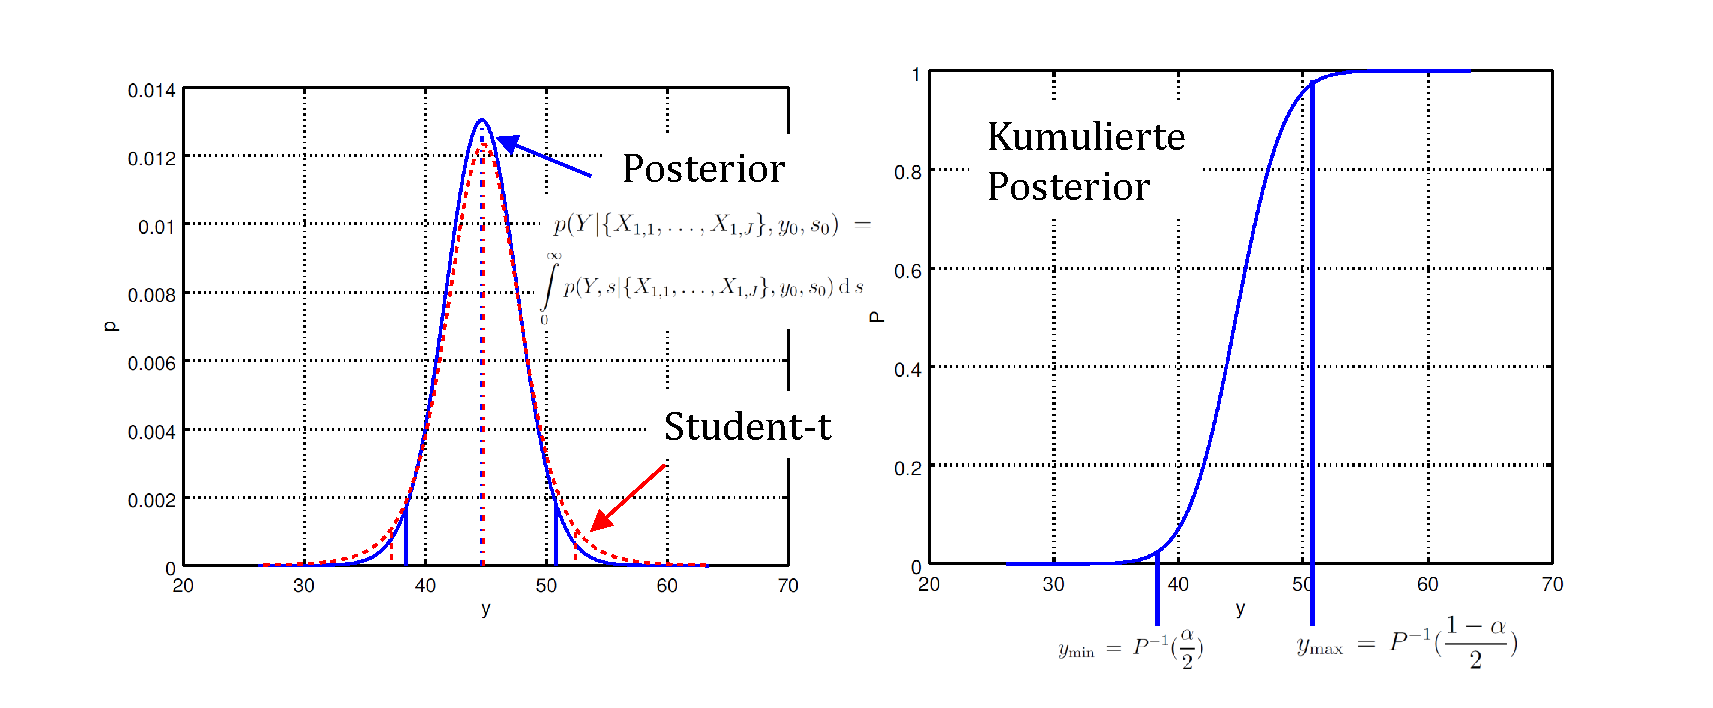
\includegraphics[width=160mm]{12_vorlesung_GUMS2/media/Ueberdeckungsintervall_0.pdf}
\caption{\label{VergleichsBeispiel}Wahrscheinlichkeitsdichtefunktionen und kumulierte Posterior
für die Bestimmung des Überdeckungsintervalls einer indirekten Messgröße}
\end{center}
\end{figure}
Wir berechnen für $\rho_{\mathrm{M}, \mathrm{K}} = 0$
$$
u^2(Y) \; = \;
\left(\frac{\partial}{\partial X_\mathrm{M}} X_\mathrm{M} X_\mathrm{K}
\right)^2_{\bar x_\mathrm{M}, K_0} \, s_\mathrm{M}^2 \; + \;
\left(\frac{\partial}{\partial X_\mathrm{K}} X_\mathrm{M} X_\mathrm{K}
\right)^2_{\bar x_\mathrm{M}, K_0} \, s_\mathrm{K}^2
$$
d.h.
$$
u(Y) \; = \;
\sqrt{ K_0^2 \, s_\mathrm{M}^2 \; + \; \bar x_\mathrm{M}^2 \, s_\mathrm{K}^2 }
\; = \; 4.802 \, \mathrm{E} .
$$
Die Anzahl der Freiheitsgrade berechnen wir gemäß der Satterthwaite'schen Gleichung
(\ref{EffectiveDFviele}), also
$$
\frac{u(Y)^4}{\nu_y} \; = \; \frac{K_0^4 \, s_\mathrm{M}^4}{\nu_\mathrm{M}} \; + \;
\frac{\bar x_\mathrm{M}^4 \, s_\mathrm{K}^4}{\nu_\mathrm{K}}
$$
d.h.\ mit $\nu_\mathrm{K} = 45$, $\nu_\mathrm{M} = 8$ und mit
$K_0 = 0.0925 \, \frac{\mathrm{E}}{\mathrm{V}}$, $s_\mathrm{K}=0.009 \, \frac{\mathrm{E}}{\mathrm{V}}$,
$\bar x_\mathrm{M} = 500.83 \, \mathrm{V}$, $s_\mathrm{M} = 17.89 \, \mathrm{V}$
$$
\nu_y \; = \; u(Y)^4 \, \left( \frac{K_0^4 \, s_\mathrm{M}^4}{\nu_\mathrm{M}} \; + \;
\frac{\bar x_\mathrm{M}^4 \, s_\mathrm{K}^4}{\nu_\mathrm{K}} \right)^{-1} \; = \;
52.58 \; \approx \; 52
$$
Die Anzahl der Freiheitsgrade kann auf ganzzahlige Werte abgerundet werden, das heißt die Nachkommastellen
 unterdrückt werden, siehe GUM JCGM 100:2008, Seite 73:
\begin{quote}
NOTE 1 If the value of $\nu_\mathrm{eff}$ obtained from Equation (G.2b) is not an integer,
which will usually be the case in practice, the corresponding value of $t_\mathrm{p}$ may be found
from Table G.2 by interpolation or by truncating $\nu_\mathrm{eff}$ to the next lower integer.
\end{quote}
\begin{lstlisting}[style=Matlab]
>> tinv(0.975,52)
ans =  2.0066
>> tinv(0.975,52.58)
ans =  2.0061
\end{lstlisting}
Wir verwenden für das t-Quantil (den Erweiterungsfaktor) den Wert $k = 2.006$, in der Praxis
nimmt man dann auch einfach $k = 2$.
Gemäß GUM kann die Formel für die effektive Anzahl von Freiheitsgraden also auch wie folgt
geschrieben werden
\begin{equation}
\nu_y \; = \;  \lfloor u(Y)^4 \, \left( \sum\limits_{i=1}^N \, \frac{ (c_i \, s_i)^4}{\nu_i}  \right)^{-1} \rfloor
\label{SatterthwaiteFloor}
\end{equation}
wobei die beiden Symbole $\lfloor r \rfloor$ um die Variable $r$ geschrieben heißen, dass
die Nachkommastellen von $r$ abzuschneiden sind, was in vielen Programmiersprachen mit der
Funktion \texttt{floor} erfolgt.

Das Vertrauensintervall wird damit schließlich
$$
[36.691 \, \mathrm{E}, 55.962 \, \mathrm{E}]
$$
und das vollständige Messergebnis
$$
Y \; = \; (46.327 \pm 9.635) \, \mathrm{E} .
$$
Der Wert für die erweiterte Unsicherheit $U = 9.635 \, \mathrm{E}$ entspricht also in etwa
dem Mittelwert aus den Berechnungen aus dem bayesischen Ansatz $\frac{1}{2} (9.423 + 9.907) =  9.665$.
Abb.~\ref{VergleichsBeispiel} zeigt das Prinzip anhand eines ähnlichen Beispiels, die eingezeichneten Werte
liegen weiter auseinander, um die Intervalle besser einzeichnen zu können.

%Bevor sich die Methoden der Kolmogoroffschen Wahrscheinlichkeitsrechnung, gemeinsame Verteilungen (\textsl{joined
%probability density distributions}) und entsprechende Margnalverteilungen zu berechnen, in der Metrologie
%(JCGM-Dokumente 101 und 102) durchgesetzt hatten, teils auch wegen der höheren Anforderungen an die Rechenleistung,
%hat man sich damit beholfen, in die Unsicherheitsfortpflanzung gemäß Gl.~(\ref{UnsicherFortpflLinearisiert}) anstelle
%von Varianzen normalverteilter oder $t$-verteilter Größen für einzelne Summanden auch

%Zu dem Kalibrierfaktor hatten wir die Anzahl der Freiheitsgrade als Information vorliegen.
%Oftmals liegen {\`a}-priori Informationen zu direkten Größen vor, ohne dass die Anzahl der
%Freiheitsgrade bekannt ist und auch ohne dass genauere Informationen zur Art der Verteilung vorliegen.
%Wie wir in der letzten Vorlesung schon gelernt haben, wird in einigen Fällen angenommen, dass
%die Verteilung sogar eine Rechteckverteilung ist, das heißt dass die Werte gleichverteilt über ein
%Intervall sind. Wir haben in dem Zusammenhang den Begriff der \textbf{Ermittlungsmethode Typ B der Messunsicherheit}
%eingeführt.

Für Größen, deren Messunsicherheit nicht unmittelbar aus vorliegenden
Stichproben gewonnen wurde, so dass Stichprobenumfang und Verteilungen nicht ermittelt
werden können, wird auf Basis heuristischer Vorstellungen eine Abschätzung der Anzahl der Freiheitsgrade
vorgenommen.

In Fällen, bei denen es um Präzisionsmessungen geht, kann vielfach angenommen werden,
dass die Anzahl der Freiheitsgrade gegen unendlich konvergiert.
\begin{equation}
\lim\limits_{\nu_i \rightarrow \infty} \, \left\{ \frac{ (c_i \, s_i)^4}{\nu_i} \right\} \; = \; 0
\end{equation}
Dies ist in Anhang G, Absatz G.4.3 des GUM JCGM 100:2008 nachzulesen. Lässt sich nicht
voraussetzen, dass die Anzahl der Freiheitsgrade sehr, sehr groß ist, so wird diese
abgeschätzt. Wie bei der Satterthwaite-Gleichung selbst, wird auch hier die Varianz der Varianz
%, siehe Anhang E, Absatz E.4.2
%\begin{equation}
%\operatorname{Var}(\bar s_i) \; \approx \; \frac{1}{2 \nu} \bar \sigma_i^2 ,
%\end{equation}
%wobei $\bar s_i$ die \textbf{empirische} Standardabweichung des Mittelwertes einer Größe $X_i$
%ist und $\bar \sigma_i = Var(X_i)$ die Standardabweichung dieser Größe ist, GUM Gl (E.7).
%Die Herleitung dieses Zusammenhangs ergibt sich aus der $\chi^2$-Verteilung, siehe Vorlesung 4 vom
%13.~November, Gln (33) bis (38) und 5.~Anhang \glqq Erwartungswerte zur $\chi^2$-Verteilung\grqq :
%$\operatorname{Var}(Q) = 2 \nu$ mit
%$Q = \nu \left(\frac{s}{\sigma}\right)^2$, so dass für die Standardabweichung der Einzelwerte gilt
\begin{equation}
\nu \; \sim \; \frac{\sigma_i^2}{\operatorname{Var}(s_i)}
\label{DFvsVariance}
\end{equation}
betrachtet, siehe GUM Anhang G, Absatz G.4.2.
Die Zuverlässigkeit der als {\`a}-priori Information mitgeteilten Unsicherheit muss
abgeschätzt werden mit einem bestimmten Prozentsatz
$(1 - \alpha) \cdot 100 \, \%$. Daraus wird heuristisch in Anlehnung an den
Zusammenhang (\ref{DFvsVariance}) die Anzahl der Freiheitsgrade abgeschätzt mit
\begin{equation}
\nu \; \approx \; \frac{1}{2 \alpha^2} .
\end{equation}
Der Quotient $\alpha$ wird als relative Unsicherheit $\frac{\Delta u}{u}$ der Unsicherheit $u$
interpretiert.

Nachdem wir gesehen haben, wie handlich die Berechnungen mit der klassischen Fortpflanzung
gegenüber den Methoden mit den Wahrscheinlichkeitsdichteverteilungen ist,
fragt man sich natürlich, weshalb wir den numerischen Aufwand mit dem Berechnen der
Integrale der Wahrscheinlichkeitsdichteverteilungen betreiben.
Für dieses kleine, handliche und anschauliche Beispiel ist dies selbstverständlich nicht
gerechtfertigt. Es dient lediglich dazu, das Grundprinzip des Verfahrens zu verdeutlichen.

Bei den Aufgaben, für die die Voraussetzungen zur Berechnung der Unsicherheit einer
indirekten Messgröße gemäß Gl.~(\ref{UnsichFortpfl2}) nicht mehr gegeben sind, werden die
Verfahren mit Rechnen mit Wahrscheinlichkeitsdichteverteilungen eingesetzt.
Dies sind Verfahren die entweder auf der Multiplikation von Likelihoodverteilungen - letztlich
auf Monte-Carlo-Berechnungen gemäß dem JCGM 101-Dokument der GUM-Reihe - oder auf der
bayesischen Statistik basieren.
Die Multiplikation von Likelihoodverteilungen setzt im Gegensatz zur bayesischen Statistik eine
\textsl{scharfe} \glqq Verteilung\grqq ~für die Modellfunktion ein. Dabei wird hier mit dem Begriff
\textsl{scharfe} Verteilung eine Wahrscheinlichkeitsdichte bezeichnet, die als Normalverteilung
mit dem Grenzübergang für $\sigma_\mathrm{winzig} \rightarrow 0$ in eine dirac'sche Deltafunktion übergeht.
Den Begriff \glqq Verteilung\grqq ~setzen wir hier in Anführungsstriche, weil
so eine dirac'sche Deltafunktion der Grenzfall ist, bei dem die Verteilung keine Verteilung mehr ist,
weil die Werte scharf und nicht mehr verteilt sind.

Bei dem Beispiel (mit Gun-Octave/matalb-Skript in Anhang \ref{AnhangBayesBeispiel})
haben wir die numerischen Integrationen in
sehr schlichter Weise dadurch realisiert, dass wir die betreffenden Größen in ein Raster äquidistanter
Stützstellen diskretisiert haben und dann einfach summiert haben. Es sollte hiermit nur das Grundprinzip der
Verfahren der \textsl{kolmogoroff'schen Wahrscheinlichkeitsrechnung} aufzeigen, die auch die Basis für die
Methoden der \textsl{bayesischen Statistik} bildet.

In vielen Fällen ist es aber nicht angesagt, beim numerischen Integrieren so zu verfahren.
Das nächste Kapitel soll deshalb einen kurzen
Überblick über unterschiedliche Verfahren zur numerischen Integration liefern.


\section{Anhang: Beispiel indirekte Größe aus Produkt zweier direkter Größen}
\label{AnhangBayesBeispiel}
Gnu-Octave Code zu dem Beispiel aus Abschnitt~\ref{MUFklassischvsbayes}

%\lstset{language=Matlab}
\lstinputlisting[style=Matlab]{12_vorlesung_GUMS2/code/bayes_indirect_quantity_product.m}
